\documentclass[12pt]{article}
\usepackage[english]{babel}
\usepackage{natbib}
\usepackage{url}
\usepackage[utf8x]{inputenc}
\usepackage{amsmath}
\usepackage{graphicx}
\graphicspath{{images/}}
\usepackage{parskip}
\usepackage{fancyhdr}
\usepackage{subcaption}
\usepackage{relsize}
\usepackage{vmargin}
\setmarginsrb{3 cm}{2.5 cm}{3 cm}{2.5 cm}{1 cm}{1.5 cm}{1 cm}{1.5 cm}

\title{Statistical Pattern Recognition}								% Title
\author{94131091}								% Author
\date{\today}											% Date

\makeatletter
\let\thetitle\@title
\let\theauthor\@author
\let\thedate\@date
\makeatother

\usepackage{listings}
\usepackage{color} %red, green, blue, yellow, cyan, magenta, black, white
\definecolor{mygreen}{RGB}{28,172,0} % color values Red, Green, Blue
\definecolor{mylilas}{RGB}{170,55,241}

\lstset{language=Matlab,%
    %basicstyle=\color{red},
    breaklines=true,%
    morekeywords={matlab2tikz},
    keywordstyle=\color{blue},%
    morekeywords=[2]{1}, keywordstyle=[2]{\color{black}},
    identifierstyle=\color{black},%
    stringstyle=\color{mylilas},
    commentstyle=\color{mygreen},%
    showstringspaces=false,%without this there will be a symbol in the places where there is a space
    numbers=left,%
    numberstyle={\tiny \color{black}},% size of the numbers
    numbersep=9pt, % this defines how far the numbers are from the text
    emph=[1]{for,end,break},emphstyle=[1]\color{red}, %some words to emphasise
    %emph=[2]{word1,word2}, emphstyle=[2]{style},    
}

\pagestyle{fancy}
\fancyhf{}
\rhead{\theauthor}
\lhead{\thetitle}
\cfoot{\thepage}

\newcommand\numberthis{\addtocounter{equation}{1}\tag{\theequation}}
\newcommand{\gl}{^{>^{w_1}}_{<_{w_2}}}
\newcommand{\svector}[2]{\left[ \begin{matrix} #1 \\ #2 \end{matrix}\right]}
\newcommand{\smatrix}[4]{\left[ \begin{matrix} #1 & #2 \\ #3 & #4 \end{matrix}\right]}
\newcommand{\Pin}{\Pi_{i=1}^n}
\newcommand{\Sumn}{\Sigma_{i=1}^n}
\begin{document}

%%%%%%%%%%%%%%%%%%%%%%%%%%%%%%%%%%%%%%%%%%%%%%%%%%%%%%%%%%%%%%%%%%%%%%%%%%%%%%%%%%%%%%%%%

\begin{titlepage}
	\centering
    \vspace*{0.5 cm}
    
\includegraphics[scale = 0.8]{Imgs/logo.png}\\[1.0 cm]	% University Logo
    \textsc{\Large Computer Engineering \&\& IT Department\newline\newline Amirkabir University of Technology}\\[2.0 cm]	% University Name
%	\textsc{\large SPR\#1}\\[0.5 cm]				% Course Code
	\rule{\linewidth}{0.2 mm} \\[0.4 cm]
	{ \huge \bfseries \thetitle}\\
	\rule{\linewidth}{0.2 mm} \\[1.5 cm]
	
	\begin{minipage}{0.4\textwidth}
		\begin{flushleft} \large
			\emph{Submitted To:}\\
			Mohammad Rahmati\\
            Assoc. Professor\\
            Computer Engineering Department\\
			\end{flushleft}
			\end{minipage}~
			\begin{minipage}{0.4\textwidth}
            
			\begin{flushright} \large
			\emph{Submitted By :} \\
			Ahmad Asadi\\
            94131091\\
            Group-G1\\
            Fall-95\\
		\end{flushright}
        
	\end{minipage}\\[2 cm]
	
	
    
    
    
    
	
\end{titlepage}

%%%%%%%%%%%%%%%%%%%%%%%%%%%%%%%%%%%%%%%%%%%%%%%%%%%%%%%%%%%%%%%%%%%%%%%%%%%%%%%%%%%%%%%%%

\tableofcontents
\pagebreak
\listoffigures
\pagebreak
\listoftables
\lstlistoflistings
\pagebreak

%%%%%%%%%%%%%%%%%%%%%%%%%%%%%%%%%%%%%%%%%%%%%%%%%%%%%%%%%%%%%%%%%%%%%%%%%%%%%%%%%%%%%%%%%
\section{Plotting conditional Parzen window based density estimates}
In the Parzen window formula, variable $V$ denotes the hypercube volume which given $h = 1$ is equal to 1. So the final formula is rewritten as \eqref{eq:1-1} in which $\omega_i$ denotes the $i$th class.
\begin{equation}
\hat{p}(x|\omega_i) = \frac{1}{n}\mathlarger{\Sigma}_{j=1}^{n_i} \phi(x - x_j)
\label{eq:1-1}
\end{equation}
According to \eqref{eq:1-1}, the first class conditional density estimate of first class based on Parzen window is expressed in \eqref{eq:1-2}.
\begin{equation}
\hat{p}(x|\omega_1) = \frac{1}{5}(\phi(x - x_1) + \phi(x - x_2) + \phi(x - x_3)) =  \frac{1}{5}(\phi(x - 4) + \phi(x - 1) + \phi(x - 5))
\label{eq:1-2}
\end{equation}
And that of the second class is expressed in \eqref{eq:1-3}.
\begin{equation}
\hat{p}(x|\omega_2) = \frac{1}{5}(\phi(x - x_4) + \phi(x - x_5)) =  \frac{1}{5}(\phi(x - 3) + \phi(x - 2))
\label{eq:1-3}
\end{equation}
Figure \ref{fig:1-1} displays both Parzen window estimated likelihood as a function of x for both classes.
\begin{figure}[h]
\centering
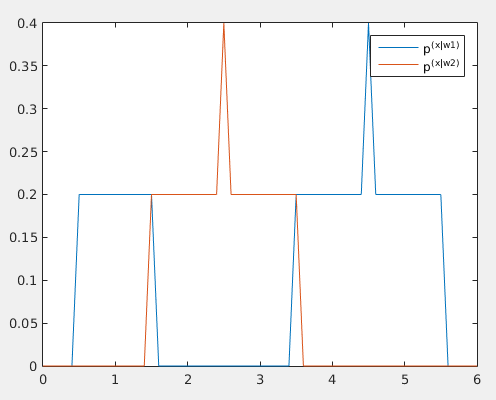
\includegraphics[scale=0.4]{Imgs/1-1.png}
\caption{Estimated likelihood of class conditional densities using Parzen window.}
\label{fig:1-1}
\end{figure}
%%%%%%%%%%%%%%%%%%%%%%%%%%%%%%%%%%%%%%%%%%%%%%%%%%%%%%%%%%%%%%%%%%%%%%%%%%%%%%%%%%%%%%%%%
\section{Plotting Parzen window estimate using Gaussian window function}
\begin{itemize}
\item
Equation \eqref{eq:2-1} represents the normal kernel.
\begin{equation}
\frac{1}{h^2}\phi(\frac{X-X_i}{h}) = (2\pi)^{-\frac{n}{2}}h^{-n}|\Sigma|^{\frac{1}{2}}exp[-\frac{1}{2}h^{-2}(X-X_i)^T\Sigma^{-1}(X-X_i)]
\label{eq:2-1}
\end{equation}
According to $\phi \sim N(0,1)$ the covariance matrix is $\Sigma = I$ and the mean vector is $\mu = 0$. The variable $n$ denoting the number of dimensions is equal to 2. So the normal kernel represented in \eqref{eq:2-1} is rewritten as equation \eqref{eq:2-2}.
\begin{equation}
\frac{1}{h^2}\phi(\frac{X-X_i}{h}) = (2\pi)^{-1}h^{-2}exp[-\frac{1}{2}h^{-2}(X-X_i)^T(X-X_i)]
\label{eq:2-2}
\end{equation}

The Parzen estimate is represented in \eqref{eq:2-3} in normal kernel case.
\begin{equation}
\hat{P} = \frac{1}{N}\mathlarger{\mathlarger{\Sigma}}_{i=1}^N \frac{1}{h^2}\phi(\frac{X-X_i}{h}) = \frac{1}{2N\pi h^2}\mathlarger{\mathlarger{\Sigma}}_{i=1}^Nexp[-\frac{1}{2}h^{-2}(X-X_i)^T(X-X_i)]
\label{eq:2-3}
\end{equation}

Using given dataset $x = \{<0.0, 1>; <0.1, 2>; <0.1, 9>; <0.3, 2>; <0.4, 1>; <0.4; 8>\}$ the Parzen estimate is computable. Figure \ref{fig:2-1} displays the estimated density using $h = 0.1$ and figure \ref{fig:2-2} displays estimated density in case of $h = 0.01$. 
\begin{figure}
\centering
\begin{subfigure}{1\textwidth}
\centering
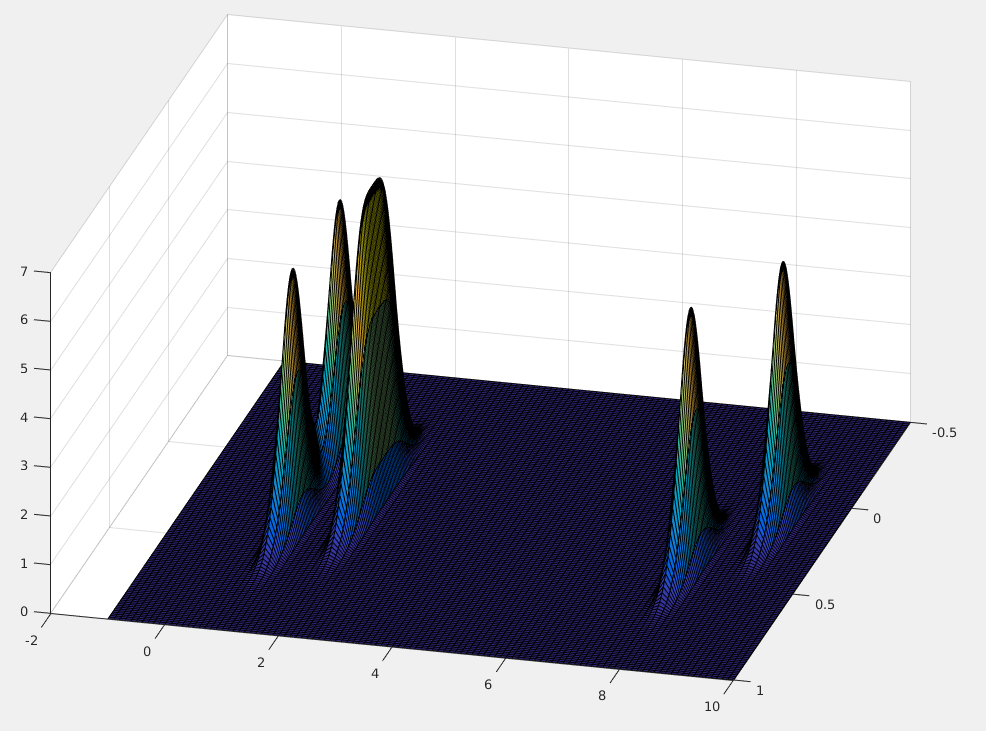
\includegraphics[scale=0.4]{Imgs/2-1.png}
\caption{Estimated density with $h = 0.1$}
\label{fig:2-1}
\end{subfigure}
\begin{subfigure}{1\textwidth}
\centering
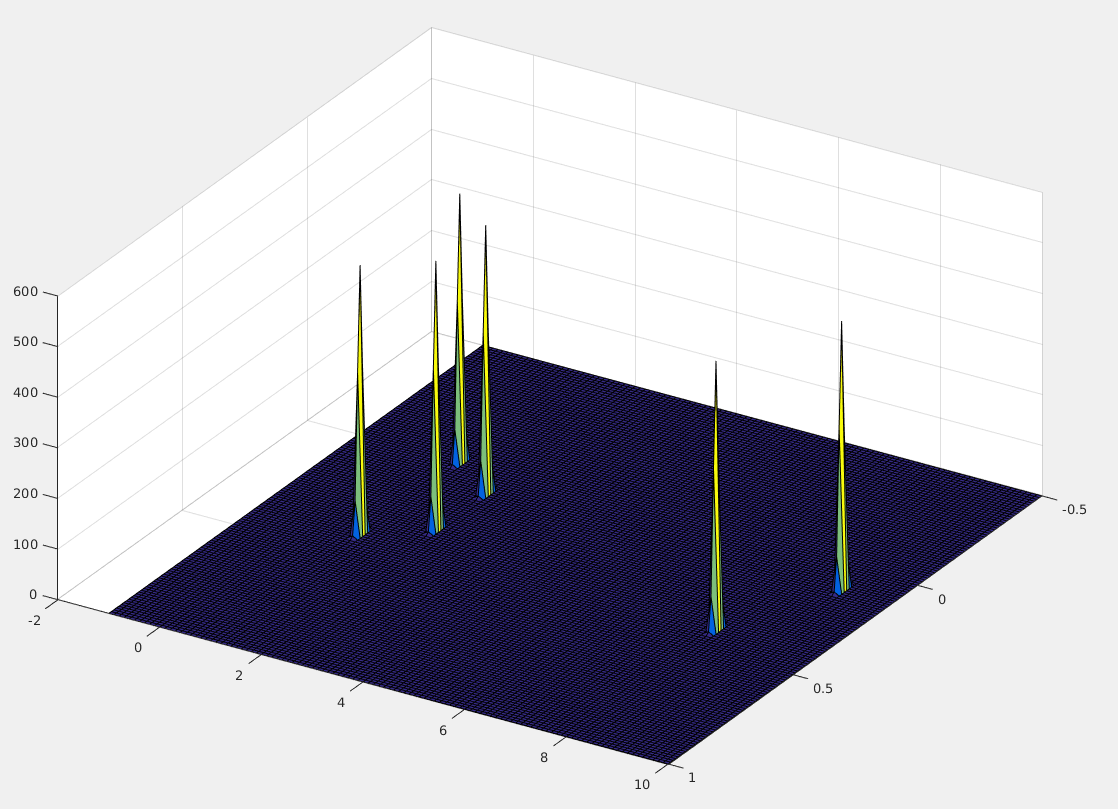
\includegraphics[scale=0.35]{Imgs/2-2.png}
\caption{Estimated density with $h = 0.01$}
\label{fig:2-2}
\end{subfigure}
\caption{Estimated density functions using Parzen Gaussian window}
\end{figure}

As it is clearly obvious, decreasing $h$ strongly makes model finer. The estimated density function is coarser when $h = 0.1$ rather than when $h = 0.01$.

\item In $K$-Nearest-Neighbour method, it is supposed to continuously increase averaging region centered at $X$ until exactly $K$ other elements locate in the region. Figure \ref{fig:2-3} displays estimated density function and its contour lines using $k$-Nearest-Neighbour algorithm with $k = 3$. As it is shown in the figure, in the regions containing 3 samples closer to each other, estimated density function has higher value rather than other regions. In addition, in the regions with 2 or less samples close to each other, although there exists a local extreme, the value of the extreme points is way lower than regions with 3 or more samples close to each other.

\begin{figure}[h]
\centering
\begin{subfigure}{.4\textwidth}
\centering
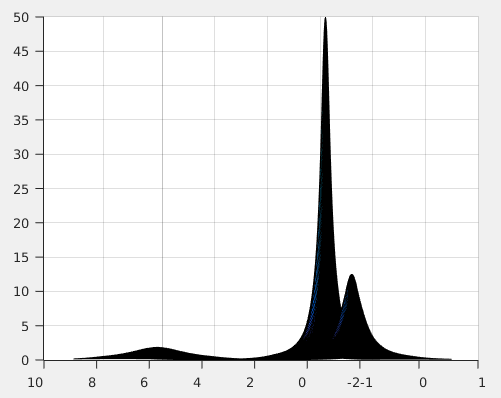
\includegraphics[scale=0.35]{Imgs/2-3.png}
\caption{Estimated density function using 3NN.}
\end{subfigure}
\begin{subfigure}{.4\textwidth}
\centering
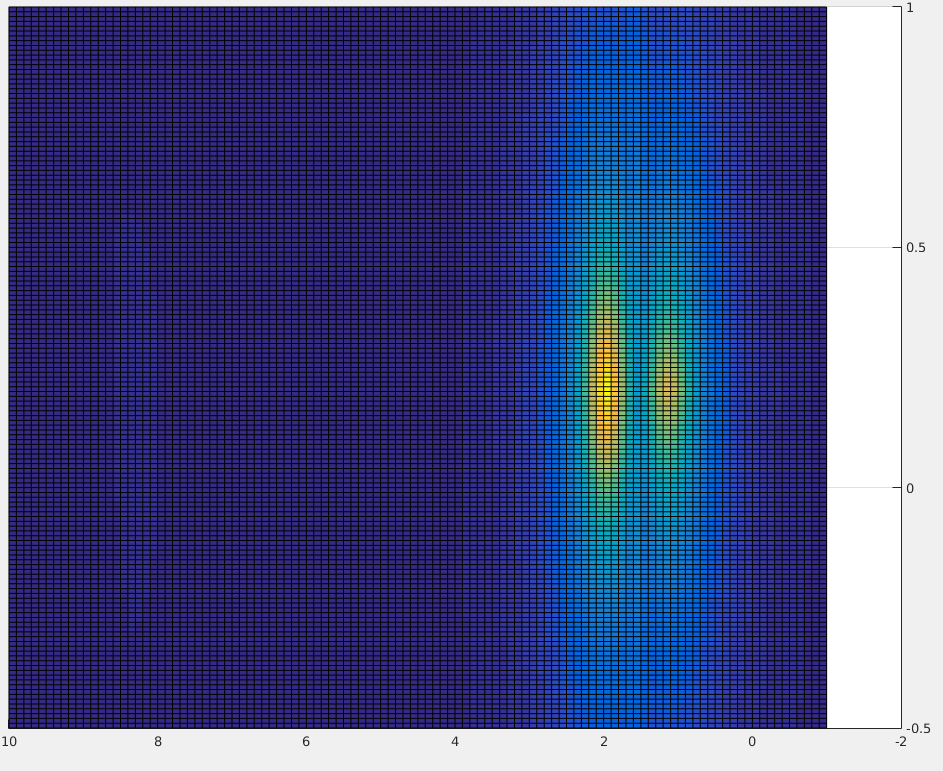
\includegraphics[scale=0.2]{Imgs/2-4.png}
\caption{Estimated density function contour lines using 3NN.}
\end{subfigure}
\caption{Estimated density function and its contour lines using 3NN according to given dataset.}
\label{fig:2-3}
\end{figure}
\end{itemize}
%%%%%%%%%%%%%%%%%%%%%%%%%%%%%%%%%%%%%%%%%%%%%%%%%%%%%%%%%%%%%%%%%%%%%%%%%%%%%%%%%%%%%%%%%
\section{Classification Error Rate Of K-Nearest-Neighbour Algorithm}
In order to compute leave-one-out cross-validation error rate of k-NN classifier, we will First classify all samples using k-NN and then calculate average on misclassified samples count. Since in the problem the exact values for real-values inputs $x$ is not given, we have assumed that the distribution of samples is like figure \ref{fig:3-1}.
\begin{figure}[h]
\centering
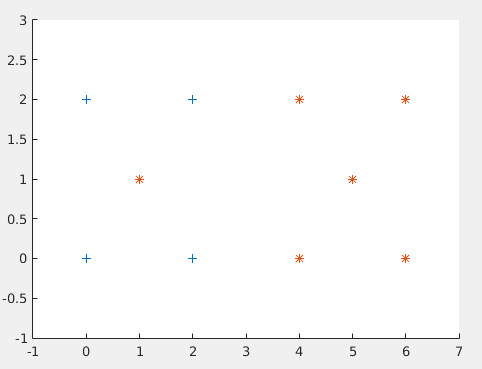
\includegraphics[scale=0.4]{Imgs/3-1.png}
\caption{Assumed distribution for given dataset in problem 3.}
\label{fig:3-1}
\end{figure}
\begin{itemize}
\item Classification using 1-NN will result in predictions displayed in figure \ref{fig:3-2} according to assumed distribution for training samples. As it is obvious in the figure, in this case, 4 samples of class $M_+$ (samples displayed by \textit{'+'} in figure \ref{fig:3-1}) and 1 sample of class $M_*$ (samples displayed by \textit{'*'} in figure \ref{fig:3-1}) are classified incorrect. So the leave-one-out cross-validation error rate of 1-NN classifier is $\epsilon = \frac{5}{10} = \frac{1}{2}$.
\item Classification using 3-NN will result in predictions displayed in figure \ref{fig:3-3} according to assumed distribution for training samples. In this case 2 samples from $M_+$ and 1 sample from $M_*$ are classified incorrect which yields leave-one-out cross-validation error rate as $\epsilon = \frac{3}{10}$.
\begin{figure}[h]
\centering
\begin{subfigure}{0.45\textwidth}
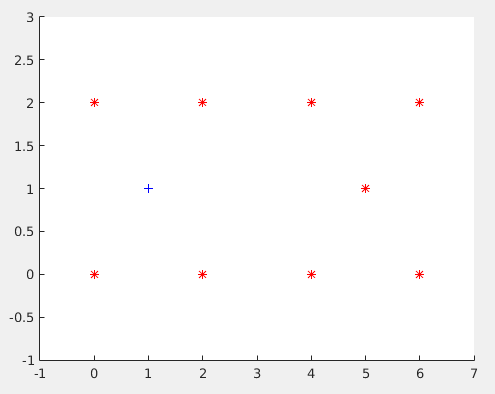
\includegraphics[scale=0.35]{Imgs/3-2.png}
\caption{Classification result using 1-NN}
\label{fig:3-2}
\end{subfigure}
\begin{subfigure}{0.45\textwidth}
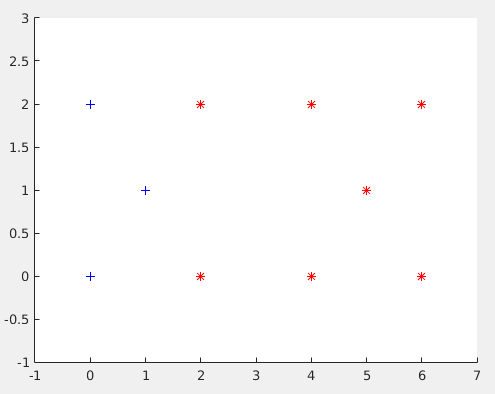
\includegraphics[scale=0.35]{Imgs/3-3.png}
\caption{Classification result using 3-NN}
\label{fig:3-3}
\end{subfigure}
\caption{Classification results of 1-NN and 3-NN classifiers on given dataset in problem 3.}
\end{figure}
\item According to a discussion in \cite{duda2012pattern} the error rate of K-NN algorithm can be calculated by equation \eqref{eq:3-1} in which $P(\omega_i|X)$ is estimated using K-NN density function estimation.
\begin{equation}
P_\epsilon = \int [1 - \Sigma_{i=1}^c P(\omega_i|X)] P(X) dX
\label{eq:3-1}
\end{equation}
In order to minimize $P_\epsilon$ represented in \eqref{eq:3-1} we should maximize $\Sigma_{i=1}^c P(\omega_i|X)$. Since there does not exist any general way to maximize $\Sigma_{i=1}^c P(\omega_i|X)$ for any possible dataset, the only working approach is to test different $K$s to get the best one. \\
In addition, there is a trade-off in model's generalizability and accuracy. To avoid overfitting, it is supposed to use a penalty function on $K$. In other words, the larger $K$, the coarser model, the higher generalizability and lower accuracy on training samples. On the other hand, the lower $K$, the more local decisions, the higher accuracy on training samples, the more effect of outliers and the less generalizability.\\
Leave-one-out cross-validation error rate could be a good measure to make a reasonable trade-off and choose a suitable $k$. It can be done as selecting $K$ in a reasonable range, calculating leave-one-out cross-validation error rate for each $K$ and selecting the $K$ which minimizes it. 
\end{itemize}
%%%%%%%%%%%%%%%%%%%%%%%%%%%%%%%%%%%%%%%%%%%%%%%%%%%%%%%%%%%%%%%%%%%%%%%%%%%%%%%%%%%%%%%%%
\section{Computer Project 1}
The listing \ref{lst:4-1} represents the MATLAB script to find the leave-one-out cross-validation error rate on training samples $D$ with labels $L$ using $K$.
\begin{lstlisting}[caption=K-NN code to compute leave-one-out cross-validation error rate on training set D with labels L using K, label=lst:4-1]
function error = KNN_LOO(D, L, K)
    error = 0 ;
    for i = 1 : size(D,1)
        X = D(i,:) ;
        dists = (repmat(X,size(D,1),1) - D).^2 ;
        dists(find(dists(:,3) ~= 0),3) = 1 ;
        dists(find(dists(:,7) ~= 0),7) = 1 ;
        dists(find(dists(:,13) ~= 0),13) = 1 ;
        dists = sum(dists.') ; 
        [~,sortedInds] = sort(dists,'ascend') ;
        knnLabels = L(sortedInds(2 : 2 + K),:) ;
        l = mode(knnLabels) ;
        if(l ~= L(i))
            error = error + 1 ;
        end
    end
    error = error / size(D,1) ;
end
\end{lstlisting}

Line 5 of listing \ref{lst:4-1} computes Euclidean distance between sample $i$th of dataset with all other points. Lines 6 to 8 are used to revise distance for nominal dimensions 3,7,13, according to data set description. Line 9 computes the distance buy summation over all dimensions. Lines 10 and 11 sorts distances in ascending order and takes top $K$ shortest distances as K-NNs. Finally the mode of labels of K-NNs defines predicted label $l$ for current sample. In lines 13 to 15 if the predicted label is not correct error will be increased one unit. Finally in line 17 the exact error will be calculated.\\
Using this function we are able to make a loop on $K$ between 1 to 10 and find the best $K$ with the smallest error rate.\\
Figure \ref{fig:4-1} represents leave-one-out cross-validation error rate for each $K$ in the range of 1 to 10. The best error rate $\epsilon = 0.3296$ has been gained with $K = 6$ in this experiment.
\begin{figure}
\centering
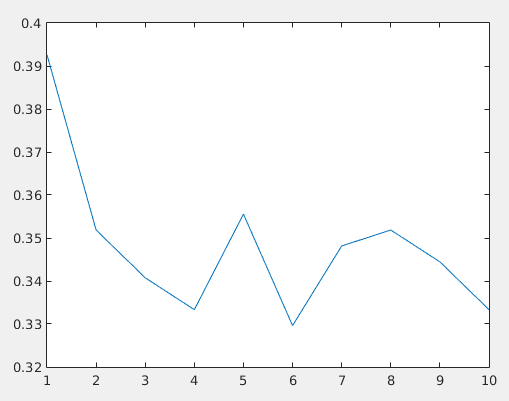
\includegraphics[scale=0.4]{Imgs/4-1.png}
\caption{The leave-one-out cross-validation error rate gained for each $K$ over given dataset in computer exercise 1.}
\label{fig:4-1}
\end{figure}
Also, table \ref{tbl:4-1} represents the averaged error rate of the algorithm for each $K$ w.r.t given dataset.
\begin{table}[h]
\centering
\caption{Reported error rates for each $K$ over given dataset in computer exercise 1.}
\label{tbl:4-1}
\begin{tabular}{c|c}
Error Rate & $K$ \\
\hline \hline 
3.925926e-01 & 1 \\
3.518519e-01 & 2 \\
3.407407e-01 & 3 \\
3.333333e-01 & 4 \\
3.555556e-01 & 5 \\
3.296296e-01 & 6 \\
3.481481e-01 & 7 \\
3.518519e-01 & 8 \\
3.444444e-01 & 9 \\
3.333333e-01 & 10 
\end{tabular}

\end{table}

The corresponding MATLAB script has been attached to the submitted file in directory \textit{src}.

%%%%%%%%%%%%%%%%%%%%%%%%%%%%%%%%%%%%%%%%%%%%%%%%%%%%%%%%%%%%%%%%%%%%%%%%%%%%%%%%%%%%%%%%%
\section{Computer Project 2}

A one-dimensional Gaussian distribution with $\mu_1 = 0$ and $\sigma_1^2 = 1$ and a two dimensional Gaussian distribution with $\mu_2 = \left[ \begin{matrix}
0 \\
0
\end{matrix}\right]$ and $\Sigma = I$ have been assumed. 30 samples from both distribution have been drawn and used for all following experiments. Note that the generated datasets have been the same in all experiments.

\begin{itemize}
\item[Parzen Kernel] :\\
In the following experiments we are going to analyse the effects of kernel function in Parzen window density estimation. We have examined 3 different kernel functions in Parzen window density estimation. equations \eqref{eq:5-1} to \eqref{eq:5-3} represent these kernels for one dimensional density estimation.
\begin{equation}
\phi_1(X) = \left\lbrace \begin{matrix}
0.5 & |X| < |\frac{h}{2}| \\
0 & otherwise
\end{matrix}\right.
\label{eq:5-1}
\end{equation}
\begin{equation}
\phi_2(X) = \left\lbrace \begin{matrix}
0.5 & G(X|\mu_1, \frac{\sigma_1^2}{10}) >= G(1|\mu_1, \frac{\sigma_1^2}{10}) \\
0 & otherwise
\end{matrix}\right.
\label{eq:5-2}
\end{equation}
\begin{equation}
\phi_3(X) = \left\lbrace \begin{matrix}
0.5 &  G(X|\mu_1, \sigma_1^2) >= G(1|\mu_1, \sigma_1^2) \\
0 & otherwise
\end{matrix}\right.
\label{eq:5-3}
\end{equation}
Note that the only difference between $\phi_2(X)$ and $\phi_3(X)$ is their variances. Figure \ref{fig:5-1} displays the estimated density functions along with real density curve.
\begin{figure}[h]
\centering
\begin{subfigure}{0.45\textwidth}
\centering 
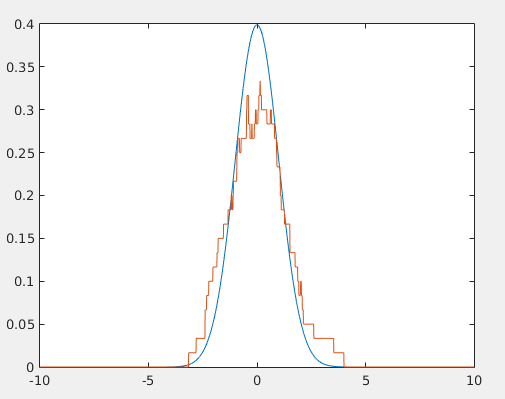
\includegraphics[scale=0.4]{Imgs/5-1.png}
\caption{Estimated density using $\phi_1(X)$}
\end{subfigure}
\begin{subfigure}{0.45\textwidth}
\centering 
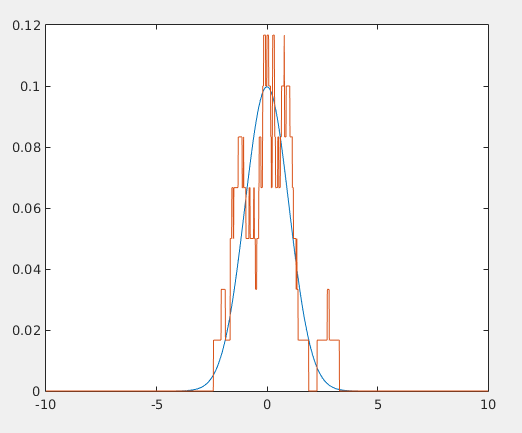
\includegraphics[scale=0.37]{Imgs/5-2.png}
\caption{Estimated density using $\phi_2(X)$}
\end{subfigure}
\begin{subfigure}{0.4\textwidth}
\centering 
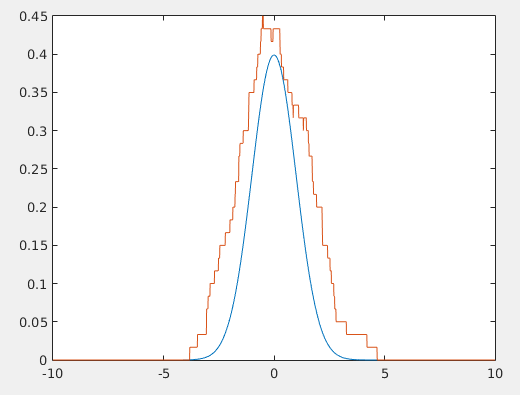
\includegraphics[scale=0.4]{Imgs/5-3.png}
\caption{Estimated density using $\phi_3(X)$}
\end{subfigure}
\caption{Effect of Parzen window kernel function to density estimation}
\label{fig:5-1}
\end{figure}

As it is clearly obvious in figure \ref{fig:5-1}, both form of kernels (Gaussian kernels $\phi2$ and $phi_3$ and linear kernel $\phi_1$) are able to estimate density function. The decrements in variances of Gaussian kernels, make estimations more spiky.\\
Assumed two dimensional Gaussian distribution has been shown in figure \ref{fig:5-2} which is used in all two dimensional experiments as the density to be estimated. Figure \ref{fig:5-3} represents the results of 2D density estimation using Parzen window with different kernels \eqref{eq:5-4} and \eqref{eq:5-5}.
\begin{equation}
\phi_4(X) = \left\lbrace \begin{matrix}
0.5 & ||X||_2^2 < |\frac{h}{2}| \\
0 & otherwise
\end{matrix}\right.
\label{eq:5-4}
\end{equation}
\begin{equation}
\phi_5(X) = \left\lbrace \begin{matrix}
0.5 & G(X|\mu_2, \Sigma) >= G(\left[ \begin{matrix} 1 \\ 1 \end{matrix}\right]|\mu_2,\Sigma) \\
0 & otherwise
\end{matrix}\right.
\label{eq:5-5}
\end{equation}
\begin{figure}[h]
\centering
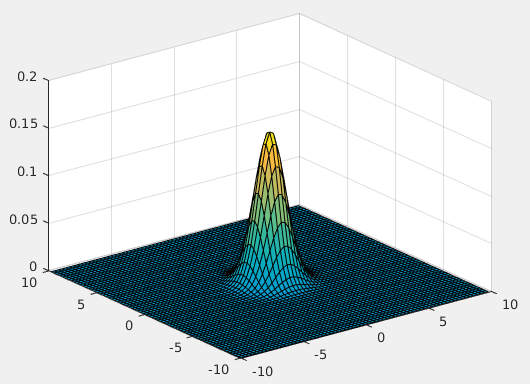
\includegraphics[scale=0.4]{Imgs/5-8.png}
\caption{Assumed 2D Gaussian distribution to be estimated.}
\label{fig:5-2}
\end{figure}
Similar to one-dimensional case, both types of kernels are able to estimate density function. In addition we can see in small number of given dataset, the normal kernel can make a better estimation of a originally normal distribution.
\begin{figure}[h]
\centering
\begin{subfigure}{0.45\textwidth}
\centering
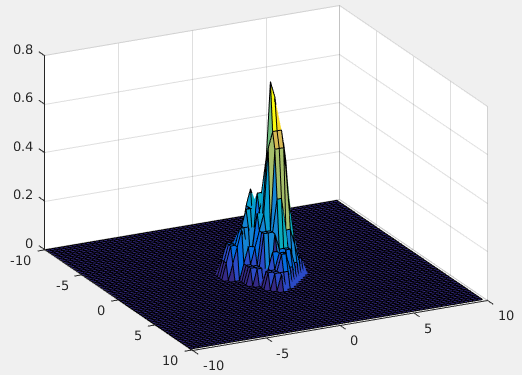
\includegraphics[scale=0.35]{Imgs/5-9.png}
\caption{Estimated density using $\phi_4$}
\end{subfigure}
\begin{subfigure}{0.45\textwidth}
\centering
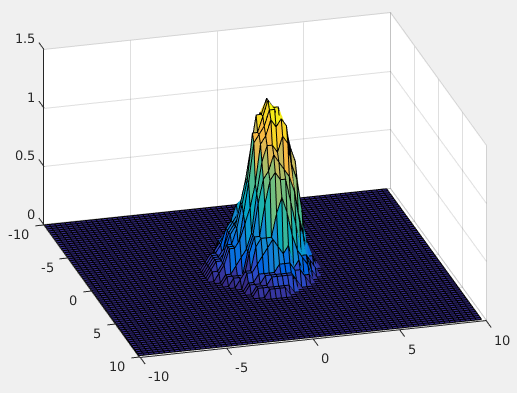
\includegraphics[scale=0.35]{Imgs/5-10.png}
\caption{Estimated density using $\phi_5$}
\end{subfigure}
\caption{Estimated 2D density function using Parzen window using different kernels.}
\label{fig:5-3}
\end{figure}

\item[Parzen Bandwidth] :\\
In the following experiments we are going to analyse the effects of bandwidth in Parzen window density estimation. The used kernel function in estimation of one-dimensional density in all cases of bandwidth, is $\phi_3(X)$. Figure \ref{fig:5-4} displays the estimation results with different bandwidths in Parzen window method.

\begin{figure}[h]
\centering
\begin{subfigure}{0.45\textwidth}
\centering
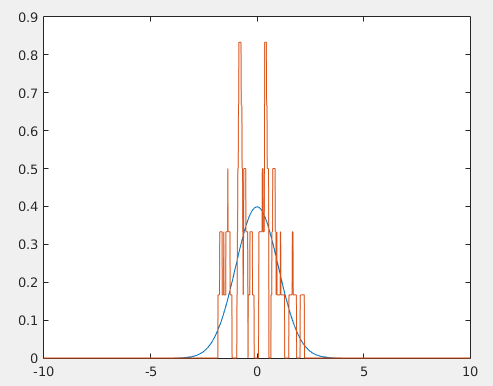
\includegraphics[scale=0.35]{Imgs/5-4.png}
\caption{Estimated density with $H = 0.1$}
\end{subfigure}
\begin{subfigure}{0.45\textwidth}
\centering
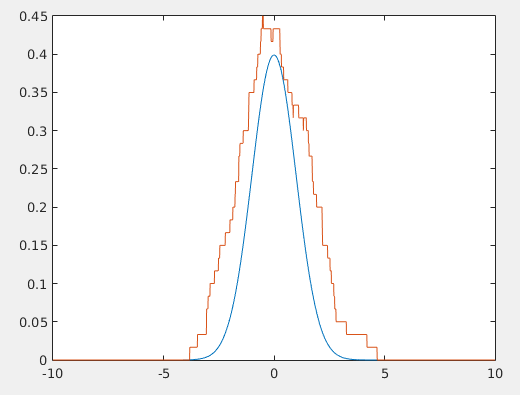
\includegraphics[scale=0.35]{Imgs/5-3.png}
\caption{Estimated density with $H = 0.5$}
\end{subfigure}
\begin{subfigure}{0.45\textwidth}
\centering
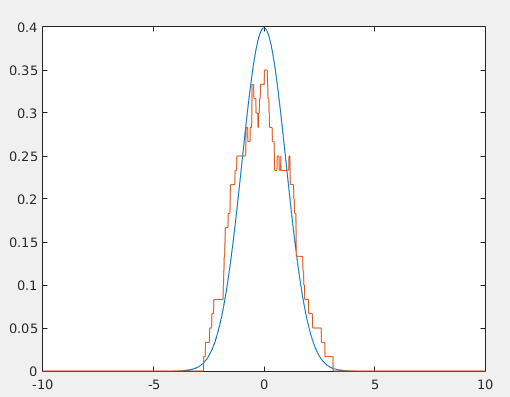
\includegraphics[scale=0.35]{Imgs/5-6.png}
\caption{Estimated density with $H = 1$}
\end{subfigure}
\begin{subfigure}{0.45\textwidth}
\centering
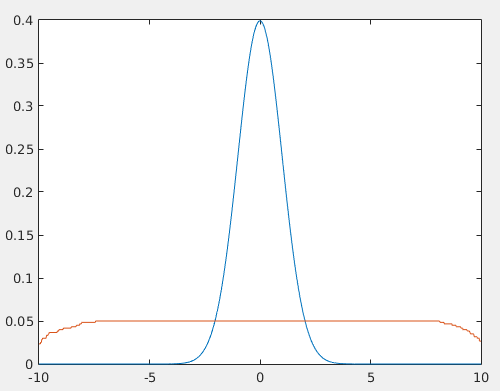
\includegraphics[scale=0.35]{Imgs/5-7.png}
\caption{Estimated density with $H = 10$}
\end{subfigure}
\caption{Estimated densities using Parzen window with different bandwidths.}
\label{fig:5-4}
\end{figure}

As it is clear in the figure \ref{fig:5-4}, the smoothness of estimated density function increases with increasing bandwidth but the accuracy decreases. Also in lower bandwidths, overfitting to the given dataset is obvious. \\
Also the results of density estimation in 2D case is similar to 1D density. Figure \ref{fig:5-5} displays the results from estimating 2D density displayed in figure \ref{fig:5-2}. In this experiment the kernel function $\phi_4$ has been used for the sake of simplicity.
\begin{figure}[h]
\centering
\begin{subfigure}{0.45\textwidth}
\centering
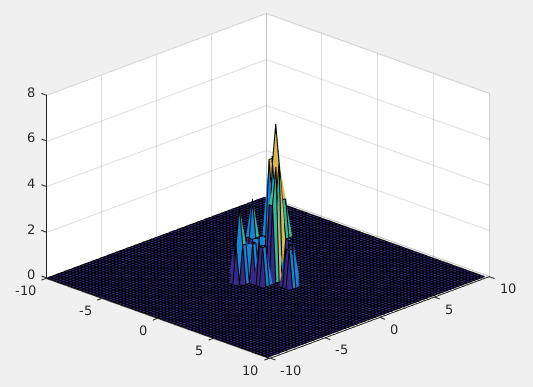
\includegraphics[scale=0.35]{Imgs/5-11.png}
\caption{Estimated 2D density with $H = 0.1$}
\end{subfigure}
\begin{subfigure}{0.45\textwidth}
\centering
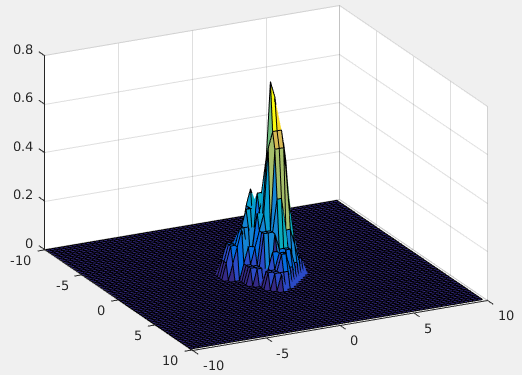
\includegraphics[scale=0.35]{Imgs/5-9.png}
\caption{Estimated 2D density with $H = 0.5$}
\end{subfigure}
\begin{subfigure}{0.45\textwidth}
\centering
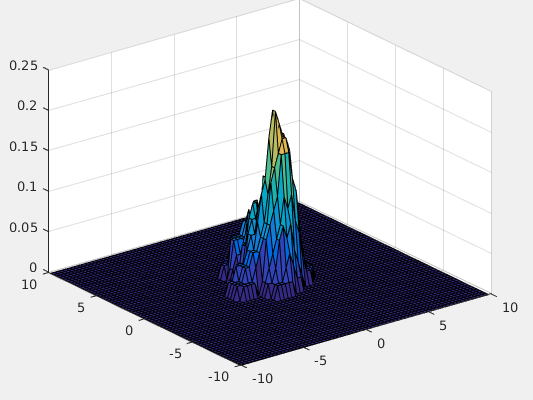
\includegraphics[scale=0.35]{Imgs/5-30.png}
\caption{Estimated 2D density with $H = 1$}
\end{subfigure}
\begin{subfigure}{0.45\textwidth}
\centering
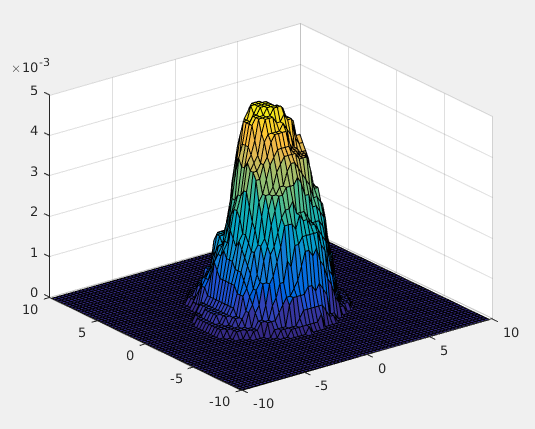
\includegraphics[scale=0.32]{Imgs/5-31.png}
\caption{Estimated 2D density with $H = 10$}
\end{subfigure}
\caption{Estimation results for 2D density estimation using Parzen window with different bandwidths.}
\label{fig:5-5}
\end{figure}
Similar to one-dimensional case, with increases in bandwidth, estimated density function gets coarser. All results and conclusions from one-dimensional case is compatible with two dimensional case, too.

\item[K in K-NN] :\\
In the following experiments we are going to analyse the effects of different $K$s in K-NN model. Increasing K in the K-NN model, tends to search for neighbours in a larger region and makes model coarser. This fact is obvious in figure \ref{fig:5-6} which illustrates the estimation results for one-dimensional density with different values for K.


\begin{figure}
\centering
\begin{subfigure}{0.45\textwidth}
\centering
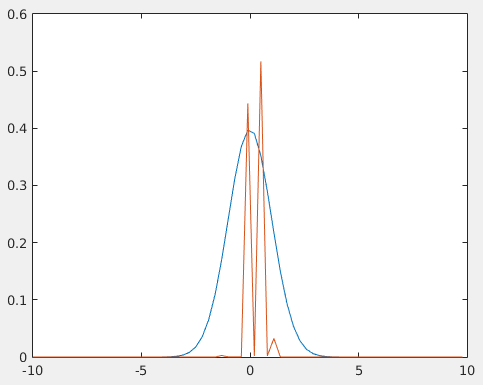
\includegraphics[scale=0.35]{Imgs/5-12.png}
\caption{Estimated density with $K = 1$}
\end{subfigure}
\begin{subfigure}{0.45\textwidth}
\centering
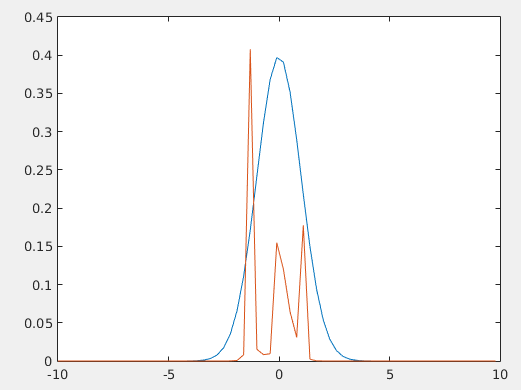
\includegraphics[scale=0.35]{Imgs/5-13.png}
\caption{Estimated density with $K = 3$}
\end{subfigure}
\begin{subfigure}{0.45\textwidth}
\centering
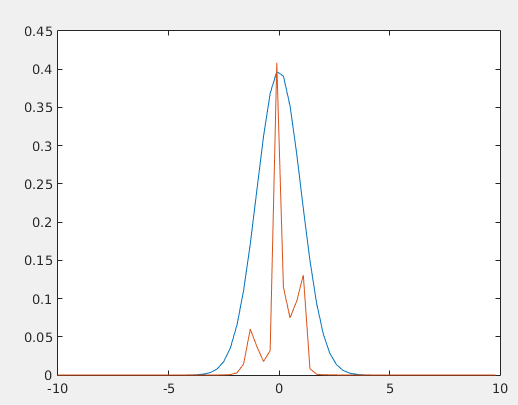
\includegraphics[scale=0.35]{Imgs/5-14.png}
\caption{Estimated density with $K = 5$}
\end{subfigure}
\begin{subfigure}{0.45\textwidth}
\centering
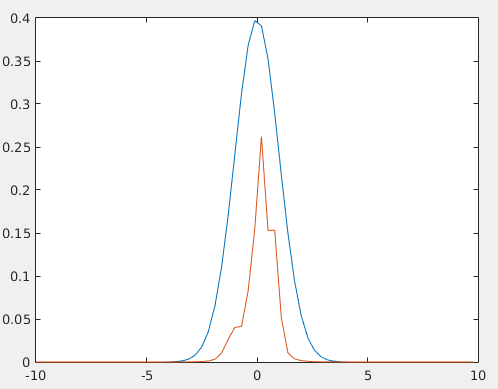
\includegraphics[scale=0.35]{Imgs/5-15.png}
\caption{Estimated density with $K = 10$}
\end{subfigure}
\begin{subfigure}{0.45\textwidth}
\centering
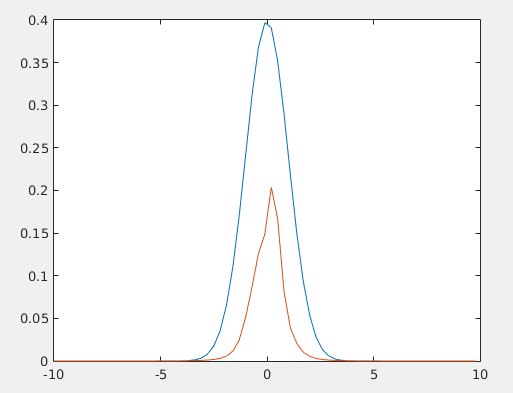
\includegraphics[scale=0.35]{Imgs/5-16.png}
\caption{Estimated density with $K = 20$}
\end{subfigure}
\caption{Estimation results for 1D density estimation using K-NN with different Ks.}
\label{fig:5-6}
\end{figure}

As it is expected, with lower values for K, the model becomes more spiky and we get near to zero estimates in a lot of wrong regions. Increasing K, results in coarser model. In the coarser models a very smooth estimation gained. The drawback of larger Ks is time wasting. More Ks result in needing more time for searching neighbours and wasted more memory. \\
The results of 2D density estimation are similar to 1D case. Figure \ref{fig:5-7} displays the density estimation for a 2D distribution. 


\begin{figure}
\centering
\begin{subfigure}{0.45\textwidth}
\centering
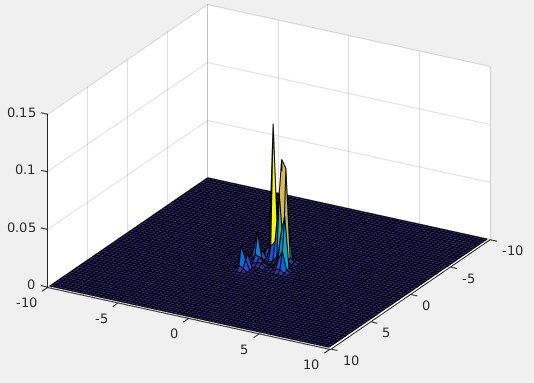
\includegraphics[scale=0.35]{Imgs/5-17.png}
\caption{Estimated density with $K = 1$}
\end{subfigure}
\begin{subfigure}{0.45\textwidth}
\centering
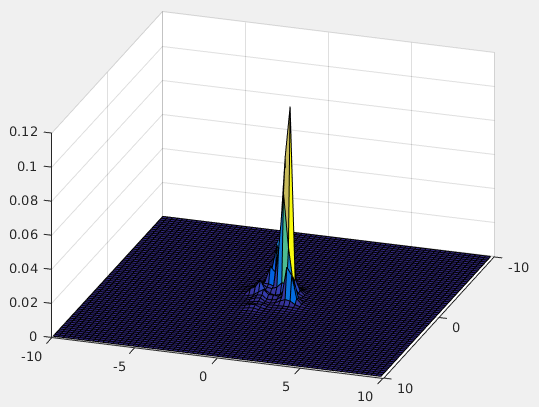
\includegraphics[scale=0.35]{Imgs/5-18.png}
\caption{Estimated density with $K = 3$}
\end{subfigure}
\begin{subfigure}{0.45\textwidth}
\centering
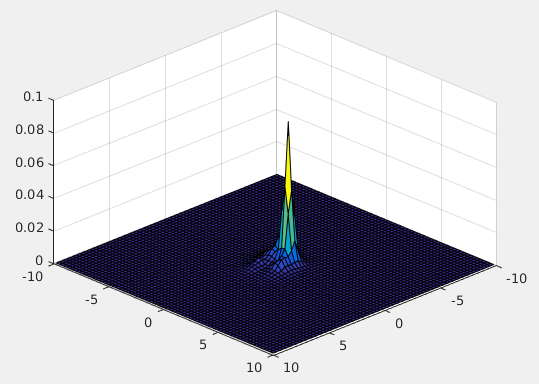
\includegraphics[scale=0.35]{Imgs/5-19.png}
\caption{Estimated density with $K = 5$}
\end{subfigure}
\begin{subfigure}{0.45\textwidth}
\centering
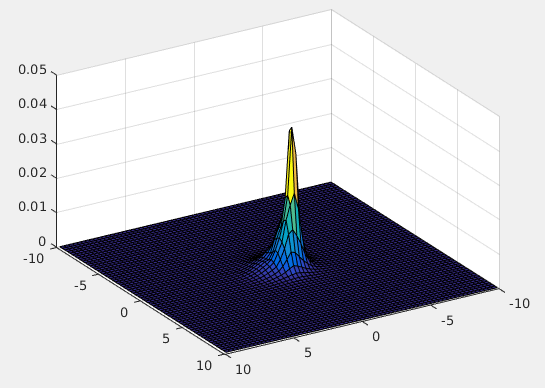
\includegraphics[scale=0.35]{Imgs/5-20.png}
\caption{Estimated density with $K = 10$}
\end{subfigure}
\begin{subfigure}{0.45\textwidth}
\centering
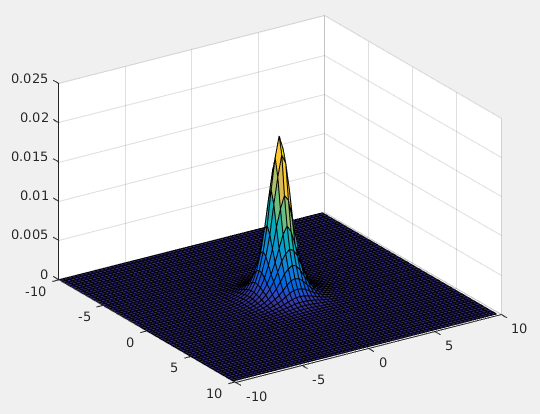
\includegraphics[scale=0.35]{Imgs/5-21.png}
\caption{Estimated density with $K = 20$}
\end{subfigure}
\caption{Estimation results for 2D density estimation using K-NN with different Ks.}
\label{fig:5-7}
\end{figure}

Similar to 1D case, the larger K, the coarser model. Effects of outliers and noisy samples will be covered better when K is larger so the resulted model is smoother and has more generalizability. When K is extremely small, zero estimates appear and points near to a noisy sample will be misclassified and the model will be overfitted to training samples set.

\item[Histogram bins] :\\
In the following experiments we are going to analyse the effects of number of bins in histogram model. When number of bins is small, the averaging regions are larger and the model is coarser. While increasing number of bins, the area of each bin will continuously be decreased and model becomes finer. In general finer models are more local and make local decisions. Also they become more overfitted to training dataset and therefore has more accuracy. \\
Figure \ref{fig:5-8} illustrates histogram density estimation with different bin counts for estimating one dimensional distribution.
\begin{figure}
\centering
\begin{subfigure}{0.45\textwidth}
\centering
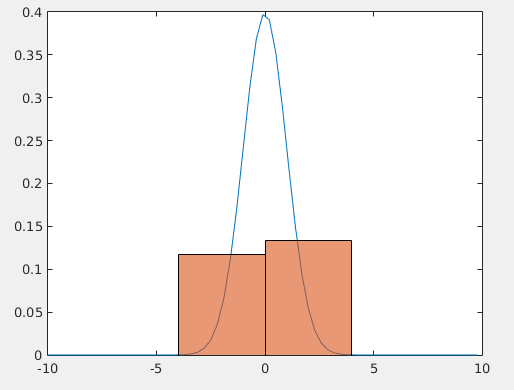
\includegraphics[scale=0.35]{Imgs/5-22.png}
\caption{Estimation using 2 bins}
\end{subfigure}
\begin{subfigure}{0.45\textwidth}
\centering
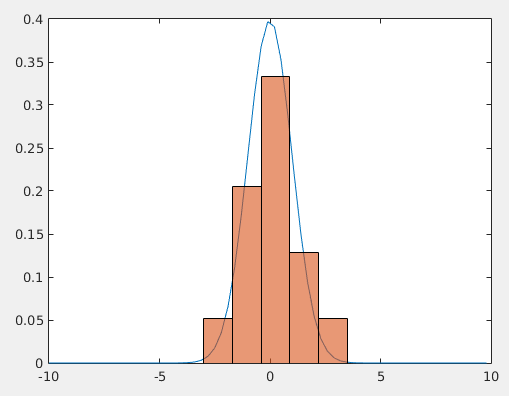
\includegraphics[scale=0.35]{Imgs/5-23.png}
\caption{Estimation using 5 bins}
\end{subfigure}
\begin{subfigure}{0.45\textwidth}
\centering
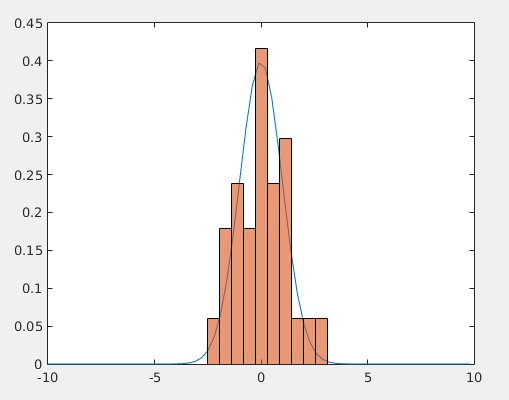
\includegraphics[scale=0.35]{Imgs/5-24.png}
\caption{Estimation using 10 bins}
\end{subfigure}
\begin{subfigure}{0.45\textwidth}
\centering
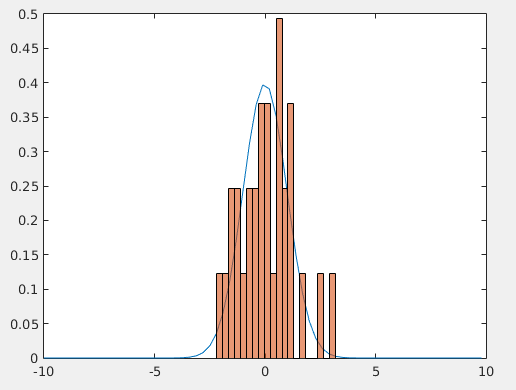
\includegraphics[scale=0.35]{Imgs/5-25.png}
\caption{Estimation using 20 bins}
\end{subfigure}
\caption{Estimated 1D density function using histogram density estimation with different bin counts.}
\label{fig:5-8}
\end{figure}

As it is clearly obvious from figure \ref{fig:5-8}, the estimated density gets finer while increasing number of bins. Model with 20 bins has more spiky points ans has zero estimates in wrong regions and is more overfitted to training dataset.\\
The effect of bin counts in 2D density estimation is exactly the same as 1D case. As it is illustrated in figure \ref{fig:5-9} the behaviour or histogram model while increasing bin counts is just like previous experiment and model with more bin counts are finer models.


\begin{figure}
\centering
\begin{subfigure}{0.45\textwidth}
\centering
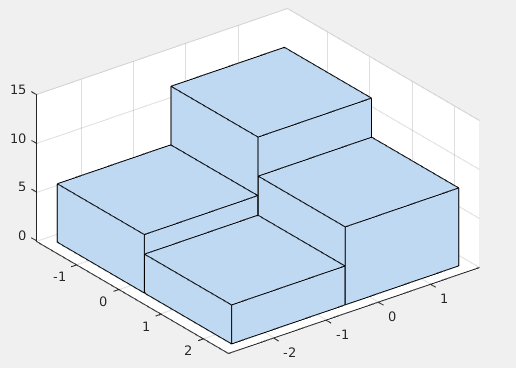
\includegraphics[scale=0.35]{Imgs/5-26.png}
\caption{Estimation using 2 * 2 bins}
\end{subfigure}
\begin{subfigure}{0.45\textwidth}
\centering
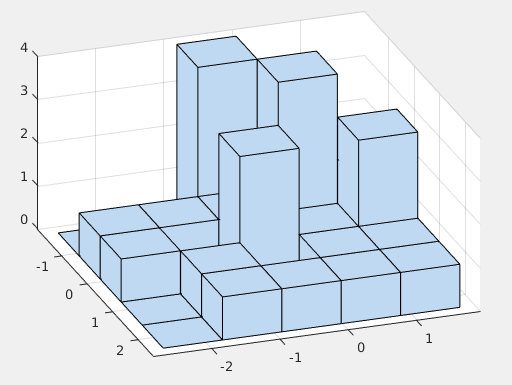
\includegraphics[scale=0.35]{Imgs/5-27.png}
\caption{Estimation using 5 * 5 bins}
\end{subfigure}
\begin{subfigure}{0.45\textwidth}
\centering
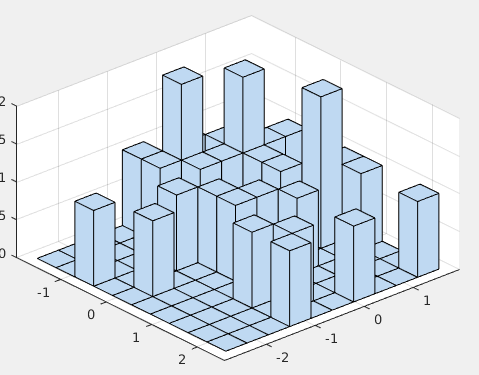
\includegraphics[scale=0.35]{Imgs/5-28.png}
\caption{Estimation using 10 * 10 bins}
\end{subfigure}
\begin{subfigure}{0.45\textwidth}
\centering
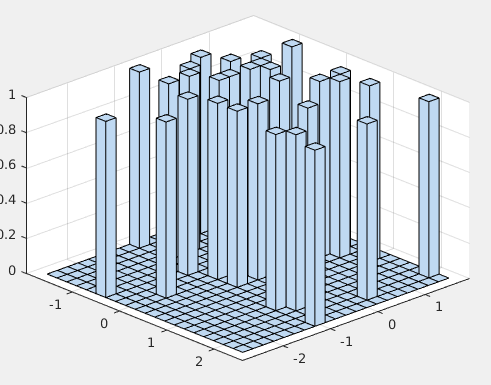
\includegraphics[scale=0.35]{Imgs/5-29.png}
\caption{Estimation using 20 * 20 bins}
\end{subfigure}
\caption{Estimated 2D density function using histogram density estimation with different bin counts.}
\label{fig:5-9}
\end{figure}


\end{itemize}


\bibliographystyle{apalike}
\bibliography{ref}
\end{document}